\documentclass[12pt,letterpaper]{article}
\usepackage[utf8]{inputenc}
\usepackage[spanish]{babel}
\usepackage{graphicx}
\usepackage[left=2cm,right=2cm,top=2cm,bottom=2cm]{geometry}
\usepackage{graphicx} % figuras
% \usepackage{subfigure} % subfiguras
\usepackage{float} % para usar [H]
\usepackage{amsmath}
%\usepackage{txfonts}
\usepackage{stackrel} 
\usepackage{multirow}
\usepackage{enumerate} % enumerados
\renewcommand{\labelitemi}{$-$}
\renewcommand{\labelitemii}{$\cdot$}
% \author{}
% \title{Caratula}
\begin{document}

% Fancy Header and Footer
% \usepackage{fancyhdr}
% \pagestyle{fancy}
% \cfoot{}
% \rfoot{\thepage}
%

% \usepackage[hidelinks]{hyperref} % CREA HYPERVINCULOS EN INDICE

% \author{}
\title{Caratula}

\begin{titlepage}
\begin{center}
\large{UNERSIDAD PRIVADA DE TACNA}\\
\vspace*{-0.025in}
\begin{figure}[htb]
\begin{center}

\includegraphics[width=8cm]{./Imagenes/logo}
\end{center}
\end{figure}
\vspace*{0.15in}
ESCUELA PROFESIONAL DE INGENIERIA DE SISTEMAS  \\

\vspace*{0.5in}
\begin{large}
TITULO:\\
\end{large}

\vspace*{0.1in}
\begin{Large}
\textbf{INFORME DE LABORATORIO No 03} \\
\end{Large}

\vspace*{0.3in}
\begin{Large}
\textbf{CURSO:} \\
\end{Large}

\vspace*{0.1in}
\begin{large}
INTELIGENCIA DE NEGOCIOS\\
\end{large}

\vspace*{0.3in}
\begin{Large}
\textbf{DOCENTE(ING):} \\
\end{Large}

\vspace*{0.1in}
\begin{large}
 Patrick Cuadros Quiroga\\
\end{large}

\vspace*{0.2in}
\vspace*{0.1in}
\begin{large}
Alumno: \\
\begin{flushleft}
Guimer Senon Coaquira Coaquira	\hfill	(2015053226) \\
\end{flushleft}
\end{large}
\end{center}

\end{titlepage}


\tableofcontents % INDICE
\thispagestyle{empty} % INDICE SIN NUMERO
\newpage
\setcounter{page}{1} % REINICIAR CONTADOR DE PAGINAS DESPUES DEL INDICE
\begin{center}
\vspace*{0.1in}
\begin{Large}
\textbf{PRACTICA DE LABORATORIO N° 03:} \\
\textbf{(Creando un Reporte Interactivo en Power BI)} \\
\end{Large}
\end{center}
\begin{document}
\section{OBJETIVO:}
\item{
Desarrollar el Informe de Labratorio 02 de Creando un Reporte Interactivo en Power BI}
\section{REQUERIMIENTOS}
\begin{itemize}

Conocimientos
Para el desarrollo de esta práctica se requerirá de los siguientes conocimientos básicos:
\\- Conocimientos básicos de administración de base de datos Microsoft SQL Server.
\\- Conocimientos básicos de SQL.

Software
Asimismo se necesita los siguientes aplicativos:
\\- Microsoft SQL Server 2016 o superior
\\- Base de datos AdventureWorksLT2016 o superior
\\- Tener los archivos de recursos del laboratorio.
\\- Power BI Desktop.
\\- Tener una cuenta Microsoft registrada en el Portal de Power Bi

\end{itemize}

\section{CONSIDERACIONES INICIALES}
\item{Generar una carpeta o directorio Power BI en un lugar accesible para guardar los resultados de la práctica.}\\
\\\\\\\\\\\\\\\\\\\\\\\\\\\\
\section{DESARROLLO}

\subsection{Actividad No 01 – DESARROLLO1}

Ejercicio 1  Conectar a datos existentes \\
	\begin{center}
	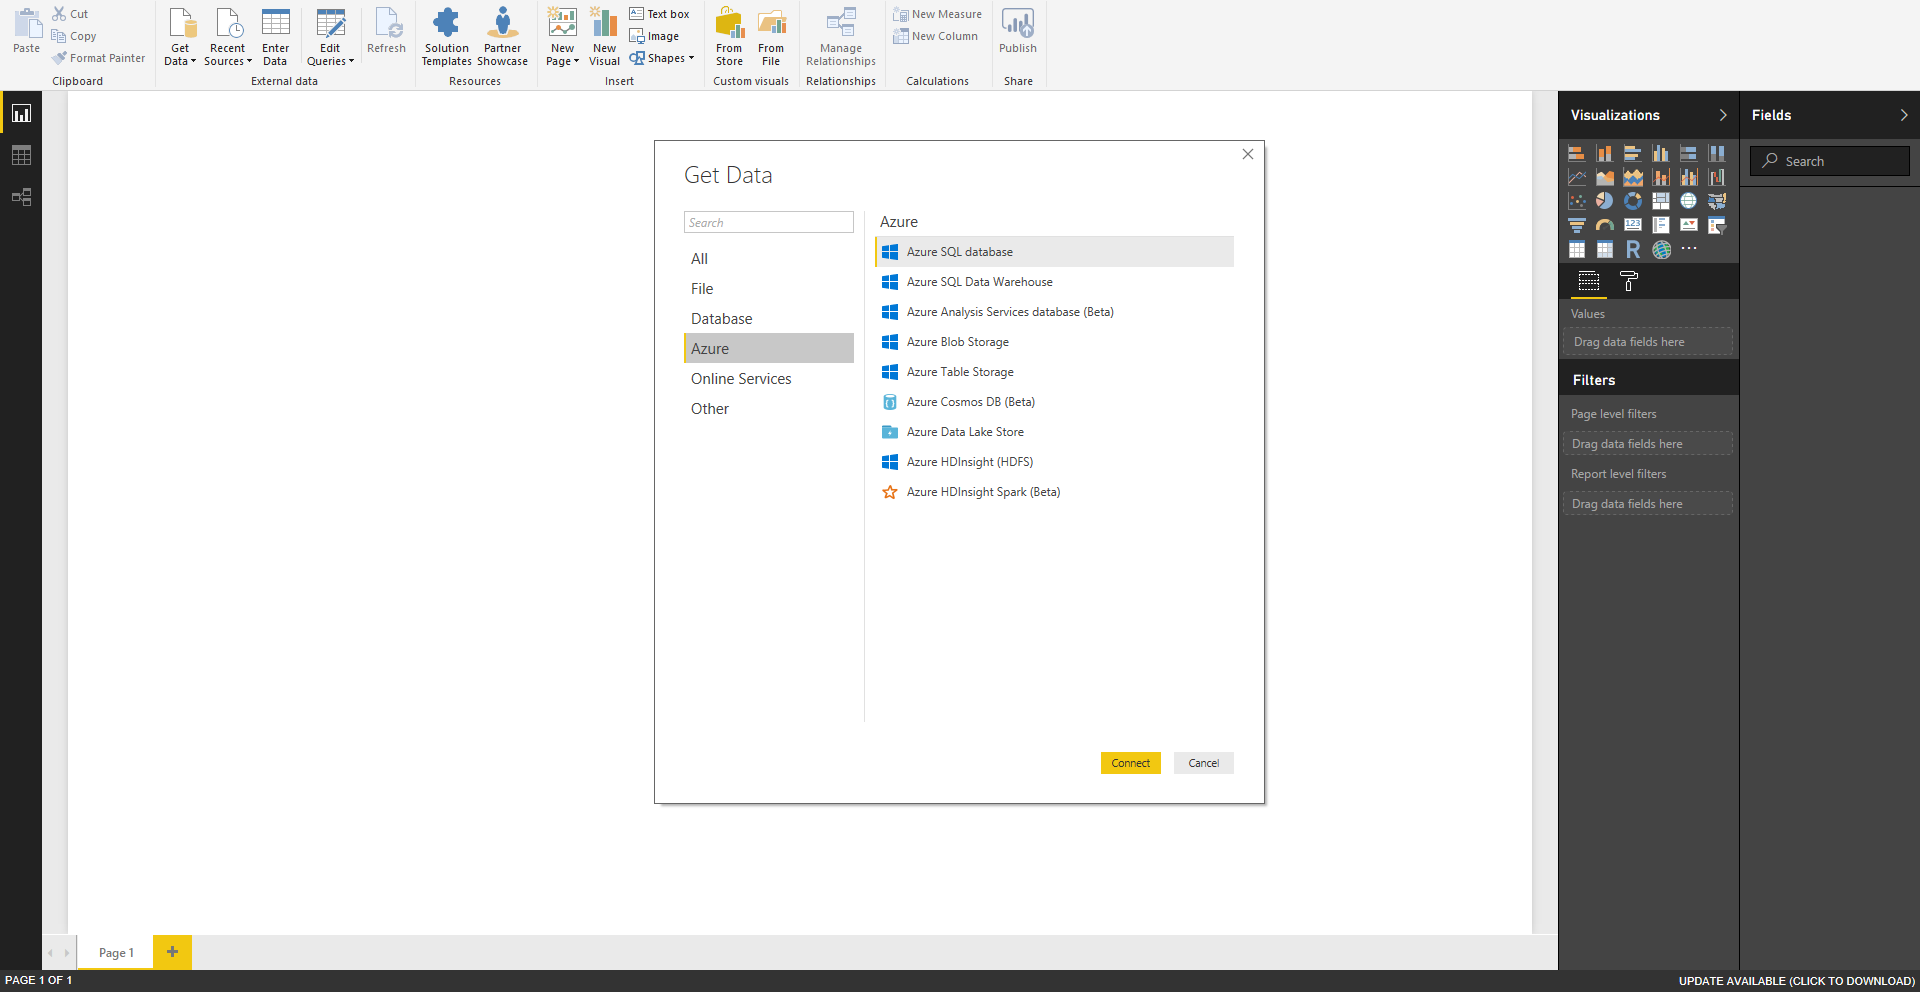
\includegraphics[width=15cm]{./Imagenes/EJER1T1(1)}
	\end{center}	

	\begin{center}
	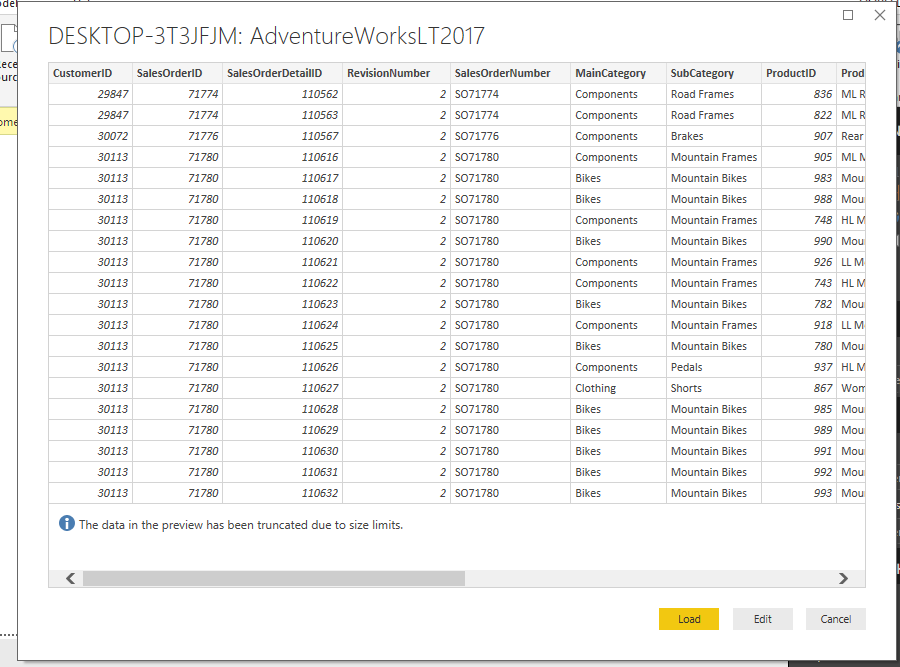
\includegraphics[width=15cm]{./Imagenes/EJER1T1(4)}
	\end{center}
	\newpage
Ejercicio 2: Shape Data\\
	\begin{center}
	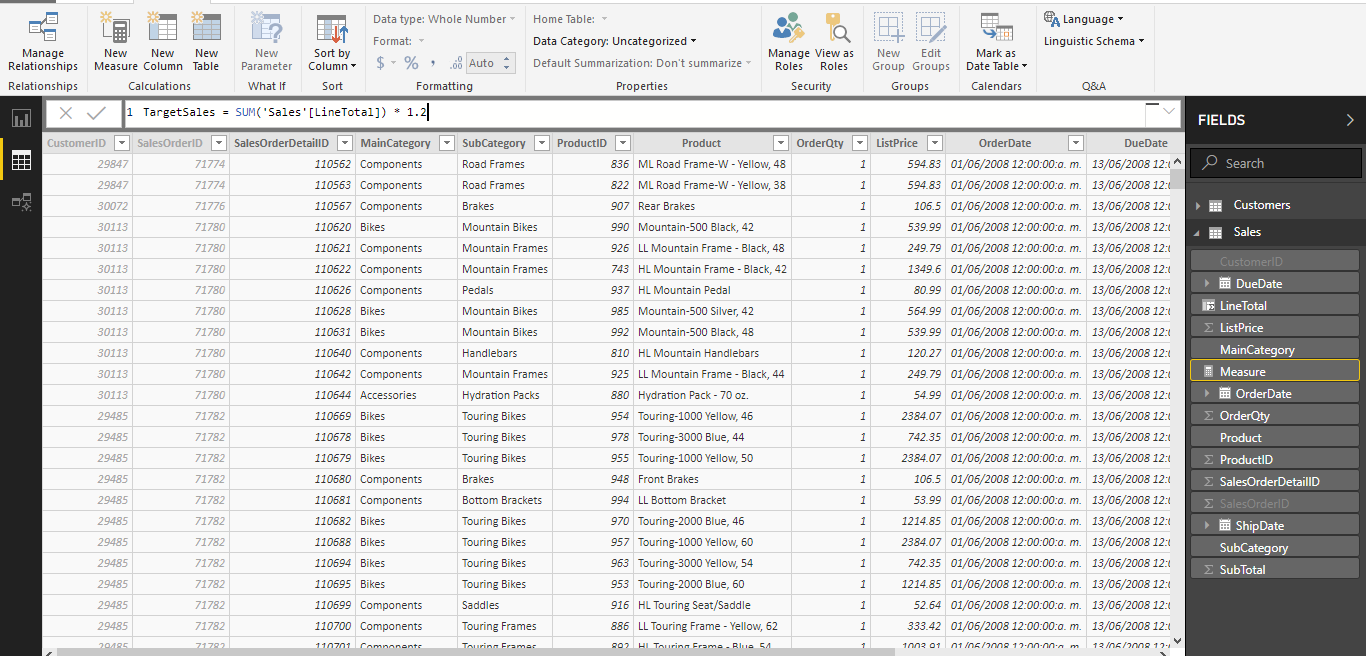
\includegraphics[width=15cm]{./Imagenes/EJER1T2(1)}
	\end{center}	

	

	\begin{center}
	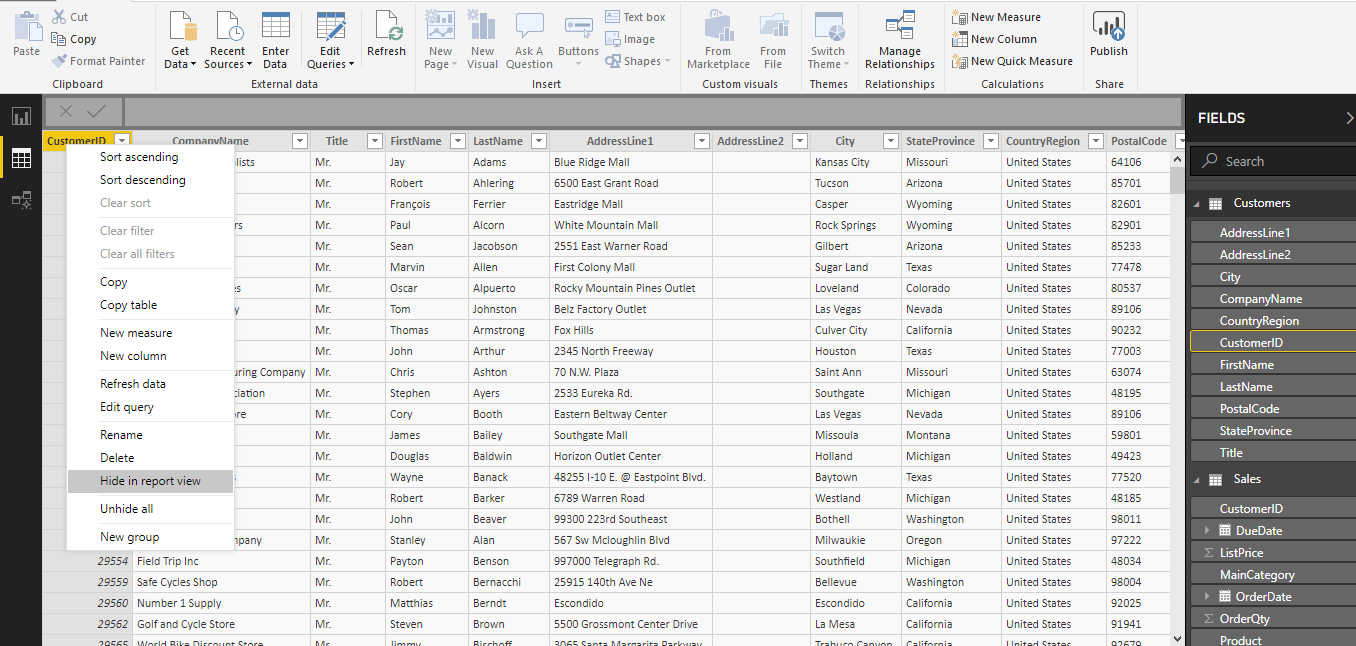
\includegraphics[width=15cm]{./Imagenes/EJER1T2(3)}
	\end{center}	
\newpage

	\begin{center}
	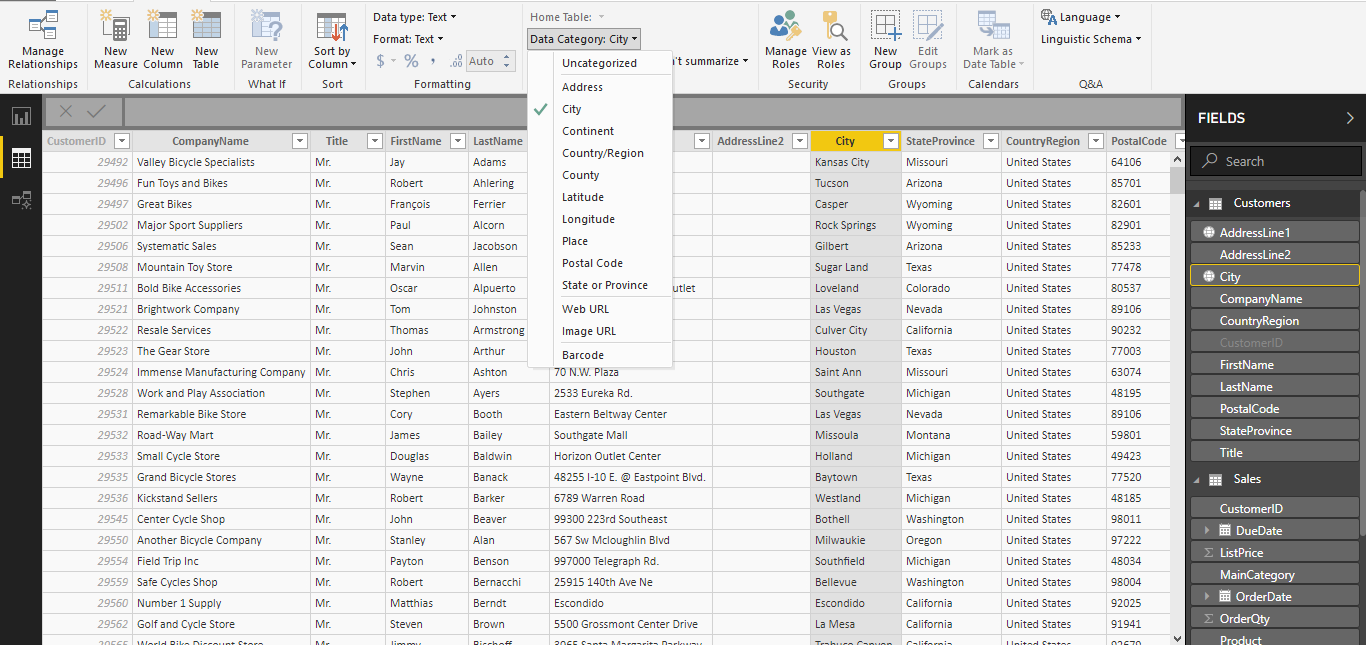
\includegraphics[width=15cm]{./Imagenes/EJER1T2(5)}
	\end{center}	


	

	\begin{center}
	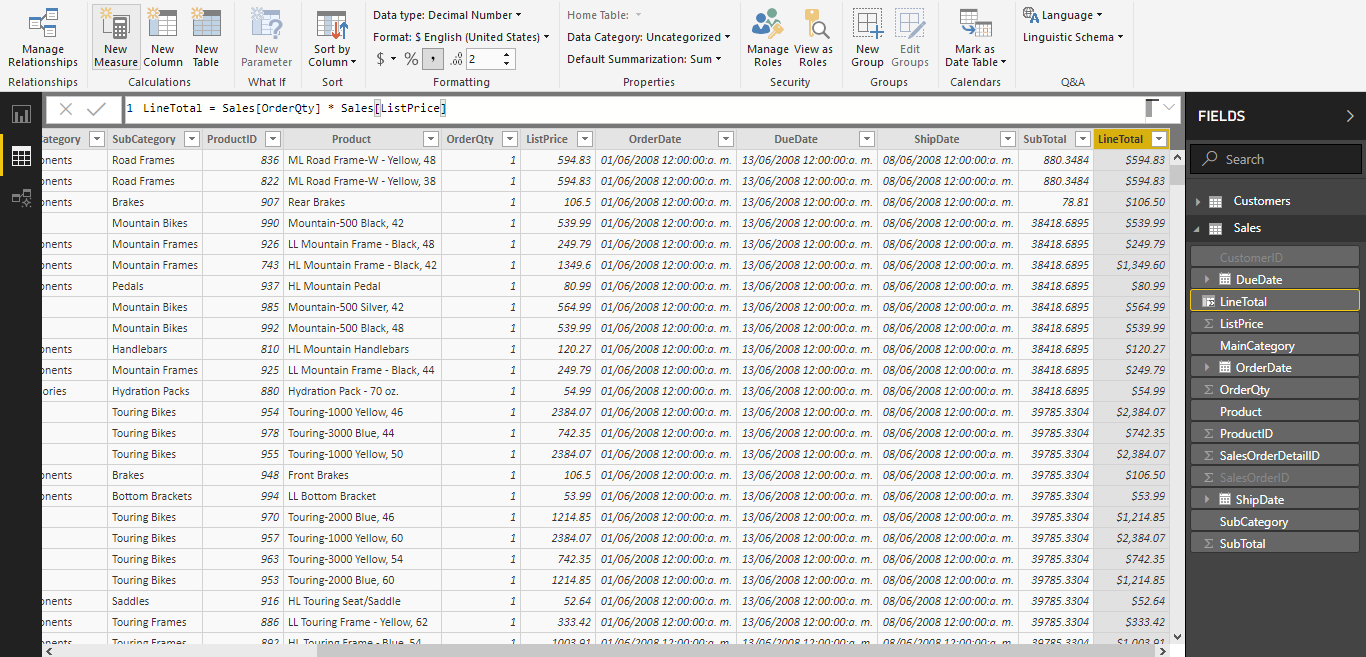
\includegraphics[width=15cm]{./Imagenes/EJER1T2(8)}
	\end{center}	
\newpage
Ejercicio 3: Combine Data\\
	\begin{center}
	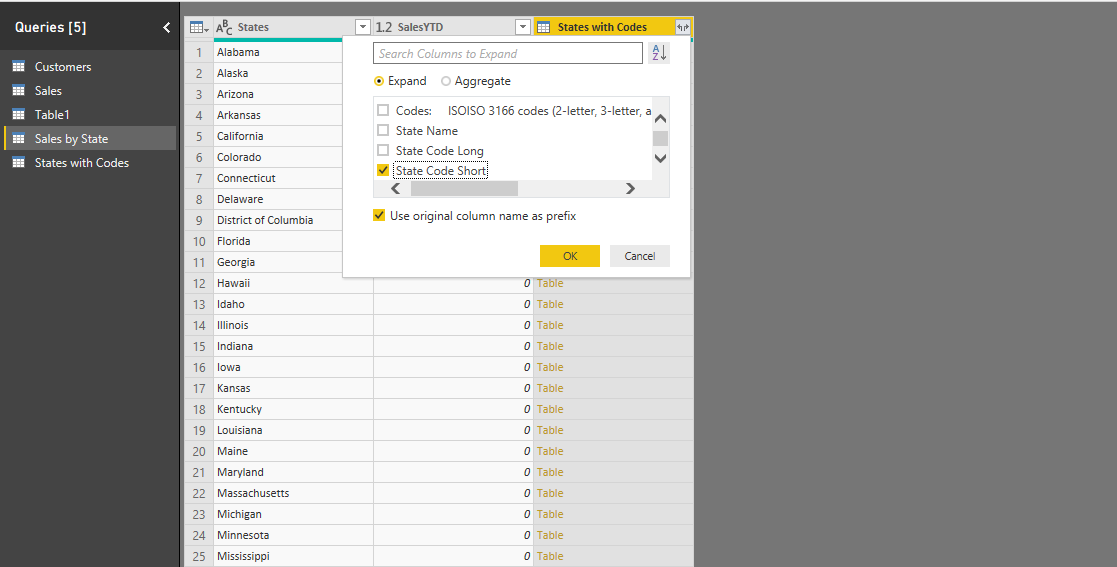
\includegraphics[width=15cm]{./Imagenes/EJER1T3(1)}
	\end{center}	

	\begin{center}
	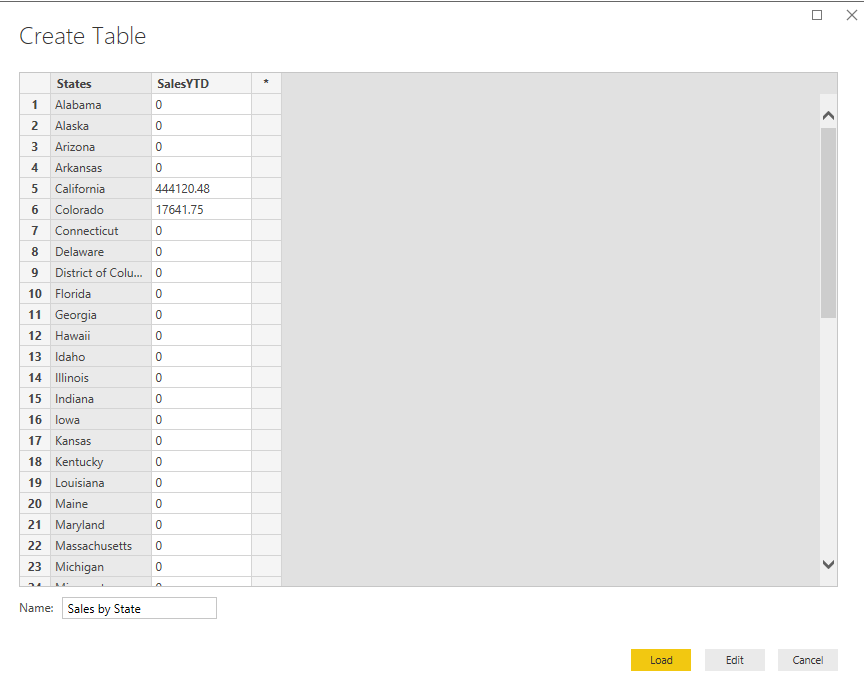
\includegraphics[width=15cm]{./Imagenes/EJER1T3(3)}
	\end{center}	
\newpage
	

	\begin{center}
	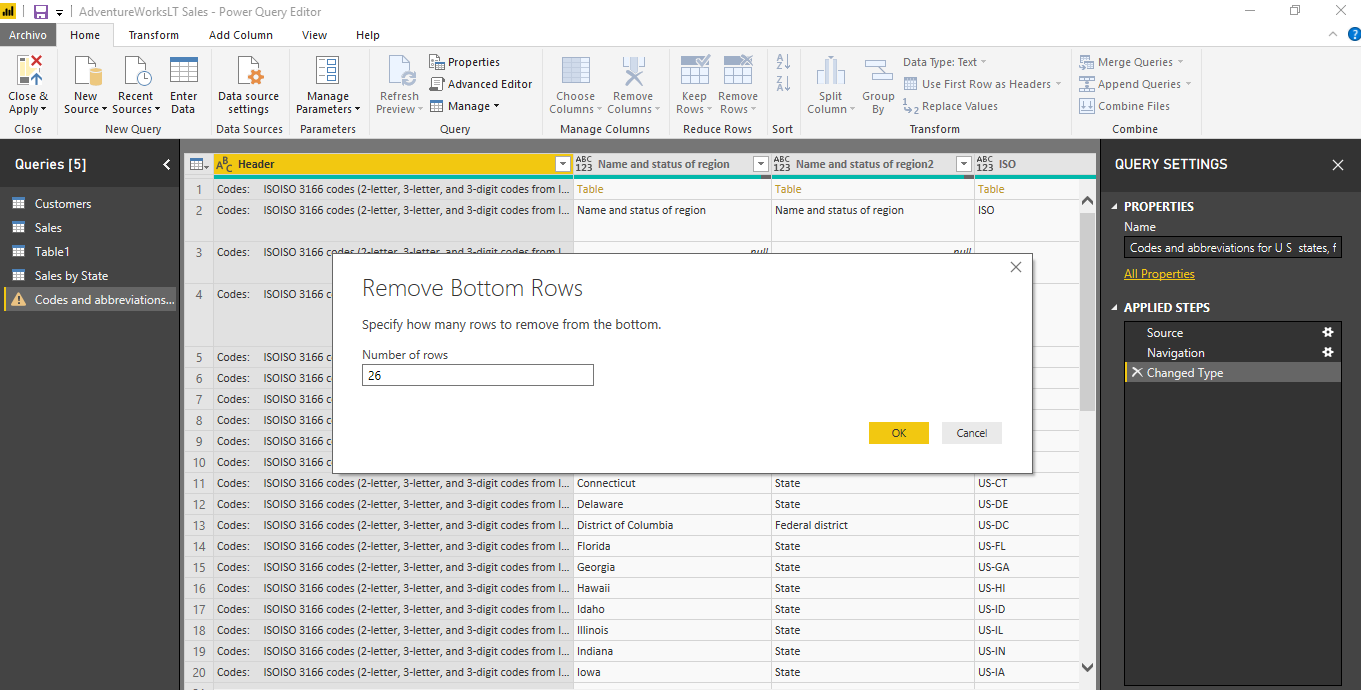
\includegraphics[width=15cm]{./Imagenes/EJER1T3(6)}
	\end{center}	
	

	\begin{center}
	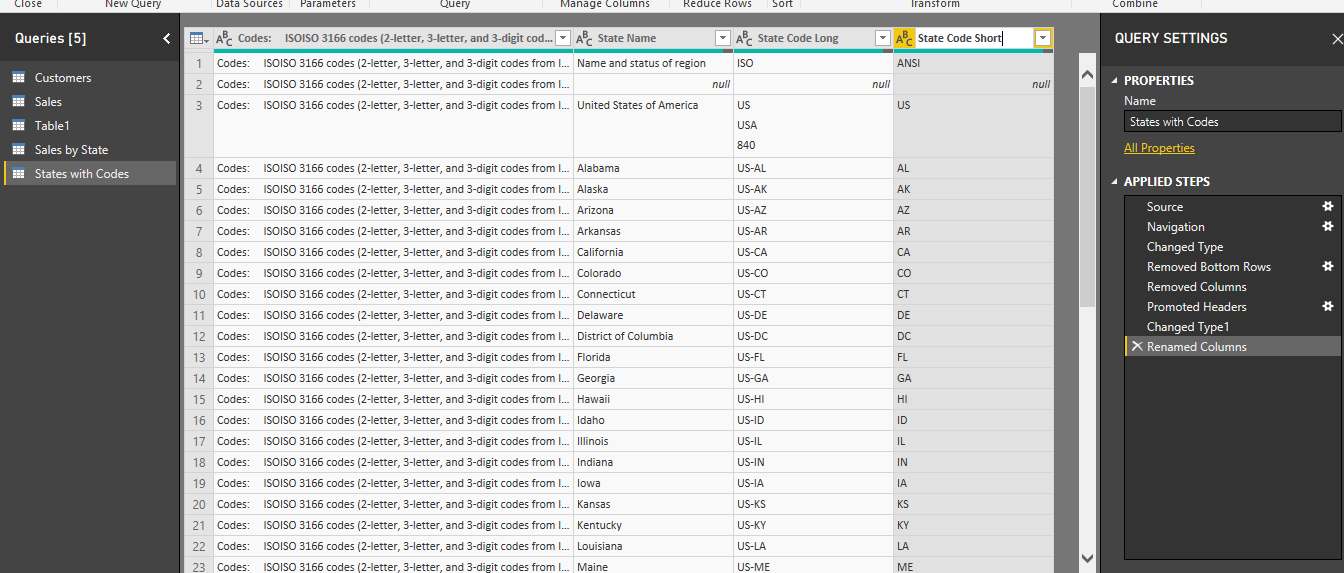
\includegraphics[width=15cm]{./Imagenes/EJER1T3(8)}
	\end{center}	
\newpage
	\begin{center}
	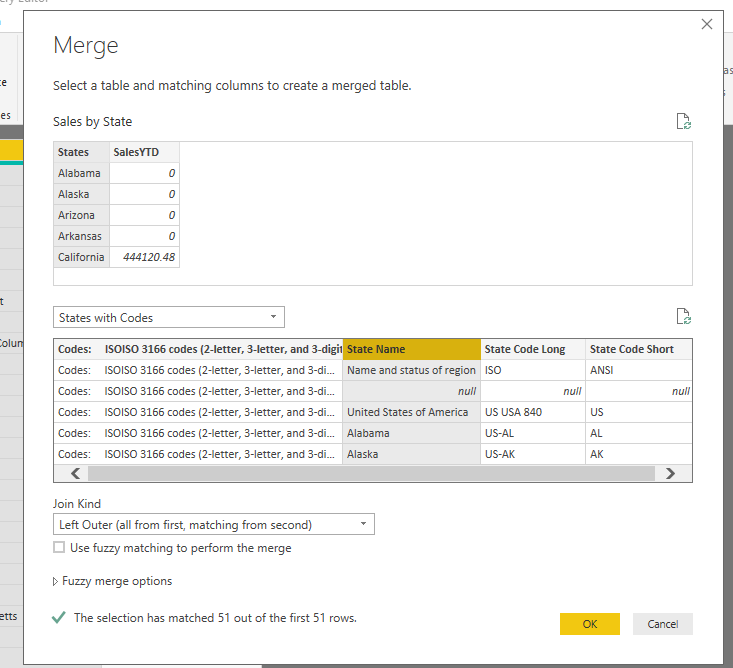
\includegraphics[width=15cm]{./Imagenes/EJER1T3(9)}
	\end{center}	




\subsection{Actividad No 02 – CONSTRUYENDO REPORTES EN POWER BI}
Ejercicio :  Crear un Gráfico \\
Ejercicio 2: Cálculos \\

	\begin{center}
	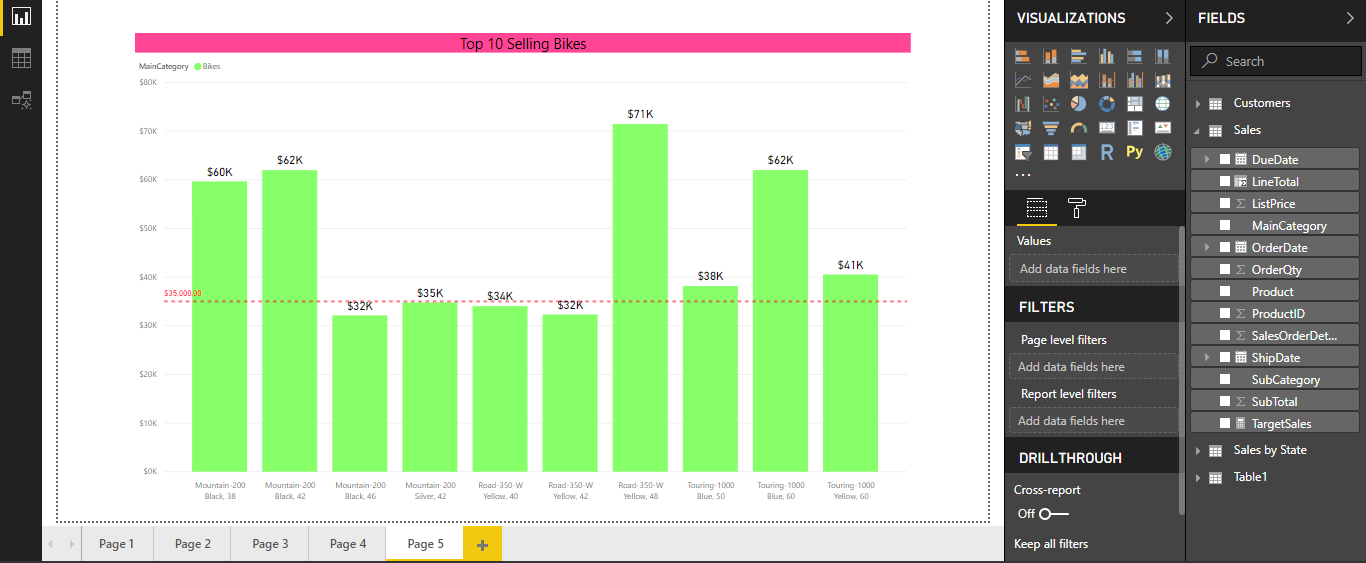
\includegraphics[width=18cm]{./Imagenes/EJER2T1(1)}
	\end{center}	

	\begin{center}
	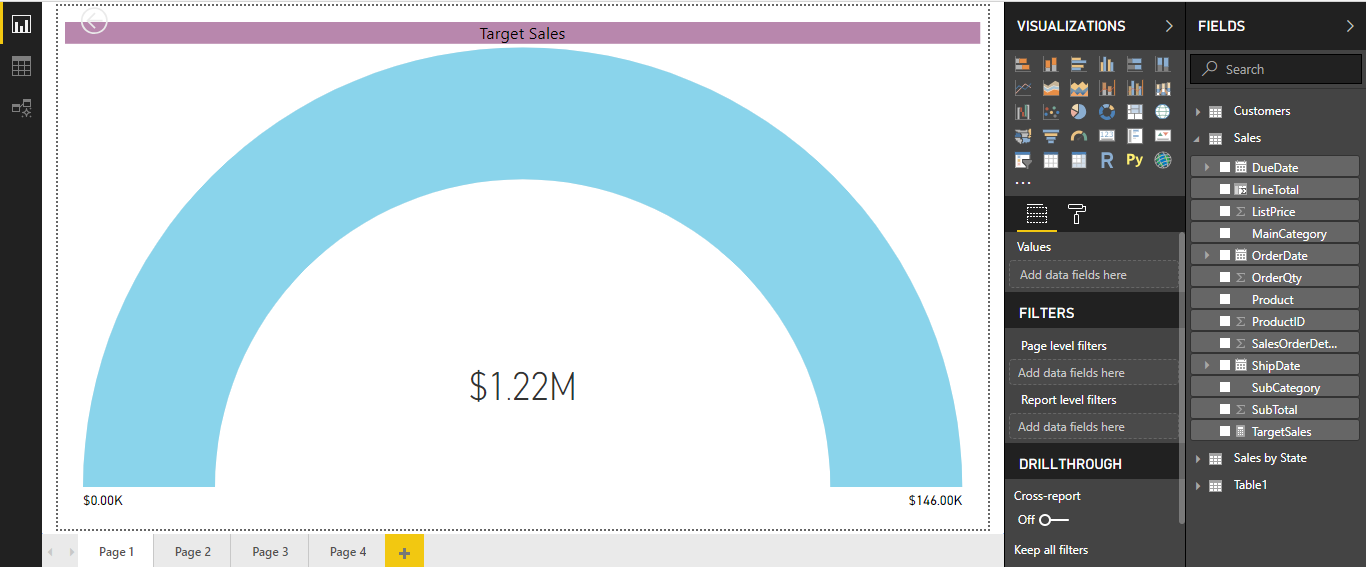
\includegraphics[width=18cm]{./Imagenes/EJER2T1(2)}
	\end{center}	

	\begin{center}
	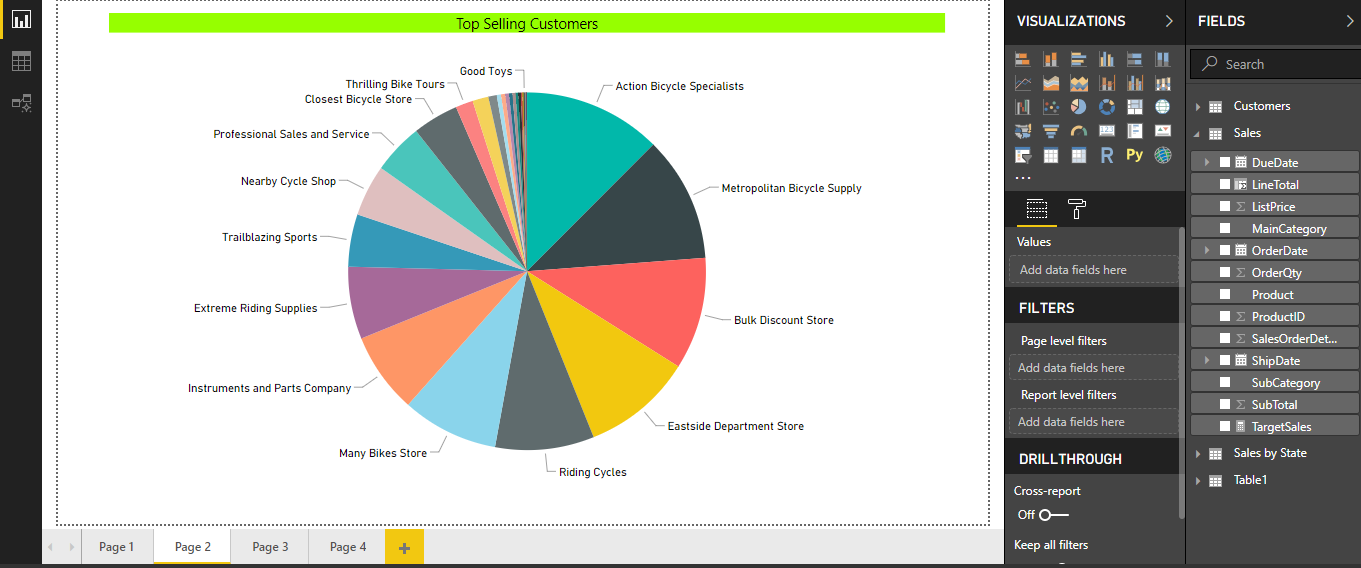
\includegraphics[width=18cm]{./Imagenes/EJER2T1(3)}
	\end{center}	

	\begin{center}
	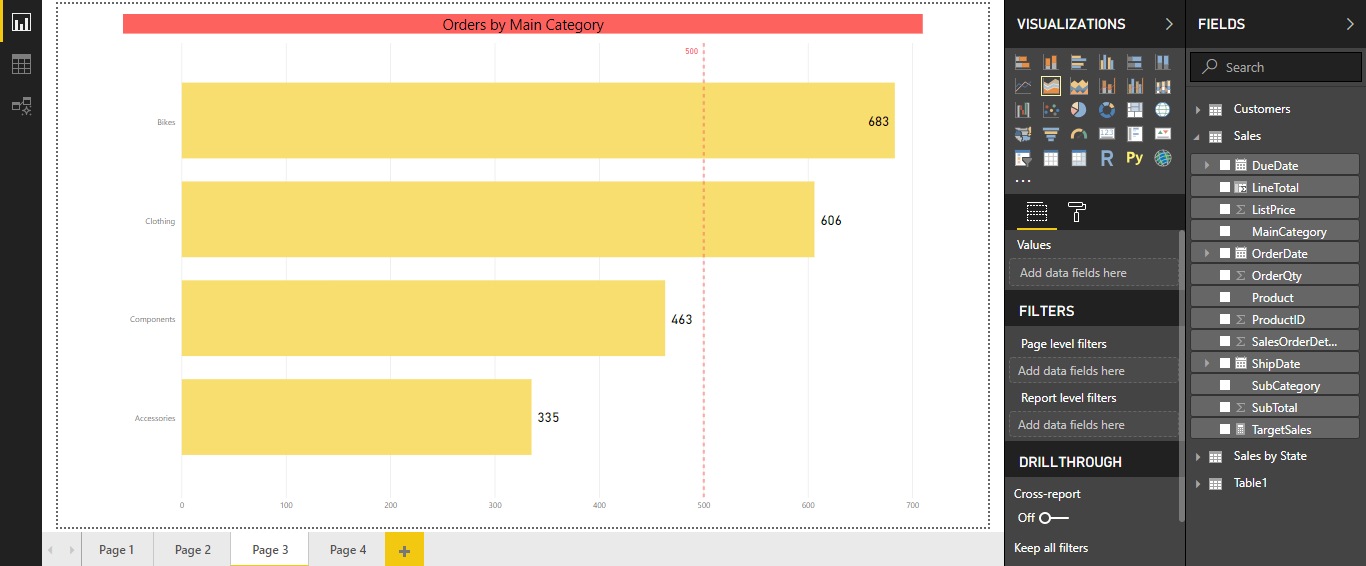
\includegraphics[width=18cm]{./Imagenes/EJER2T1(4)}
	\end{center}	
\newpage
	\begin{center}
	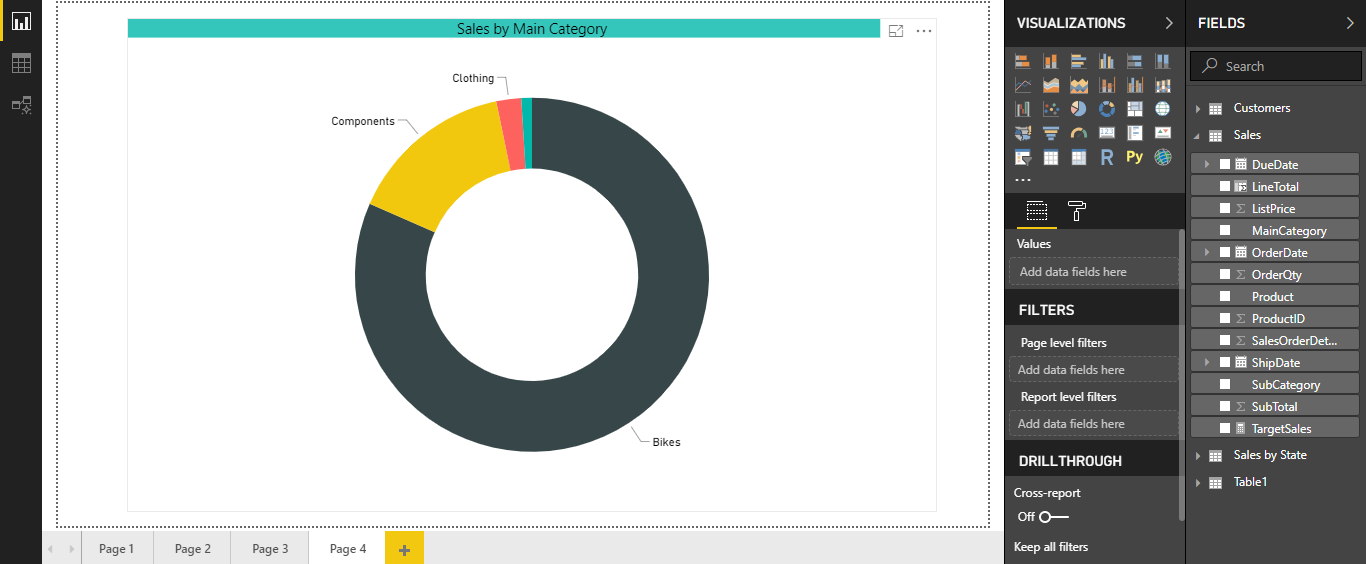
\includegraphics[width=18cm]{./Imagenes/EJER2T1(5)}
	\end{center}	

	

\subsection{Actividad No 03 –  CREATING A POWER BI DASHBOARD}

Ejercicio 3: Publish Reports from Power BI Desktop \\


	

	\begin{center}
	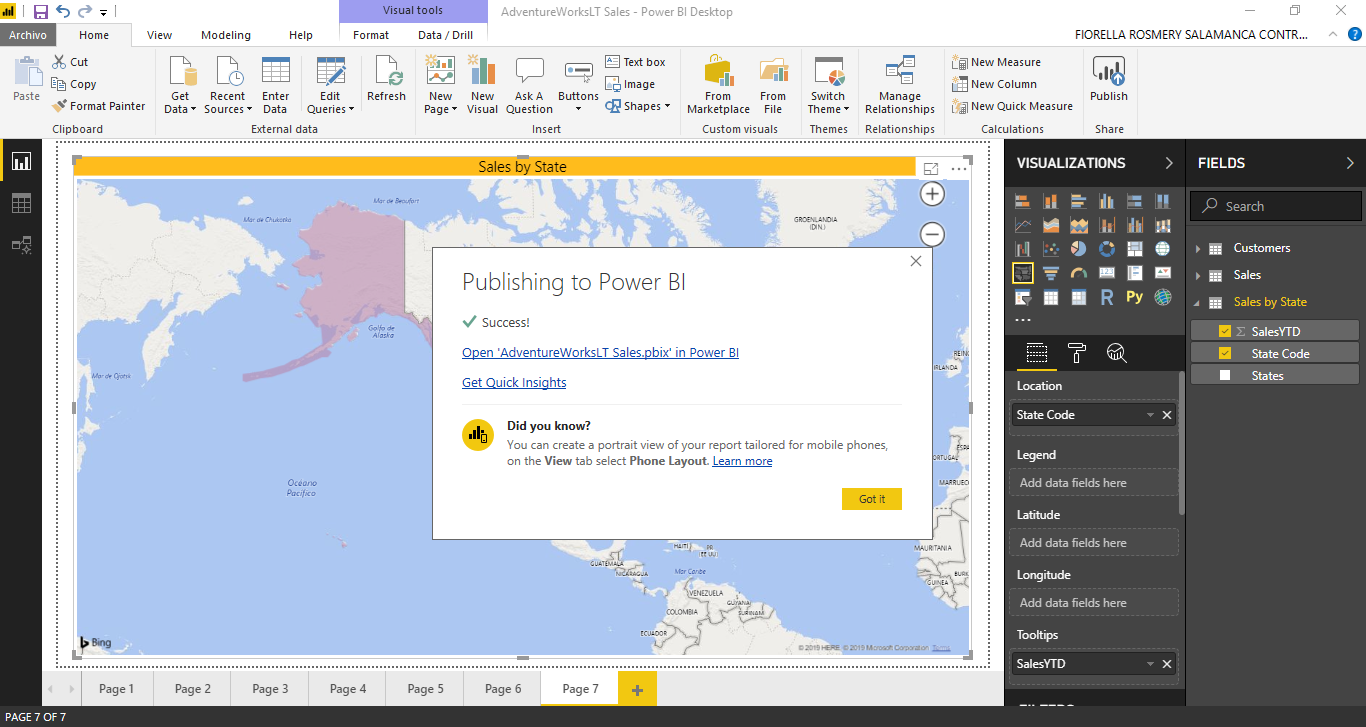
\includegraphics[width=18cm]{./Imagenes/EJER3T1(2)}
	\end{center}
\newpage	
Ejercicio 3: Create a Power BI Dashboar \\
	\begin{center}
	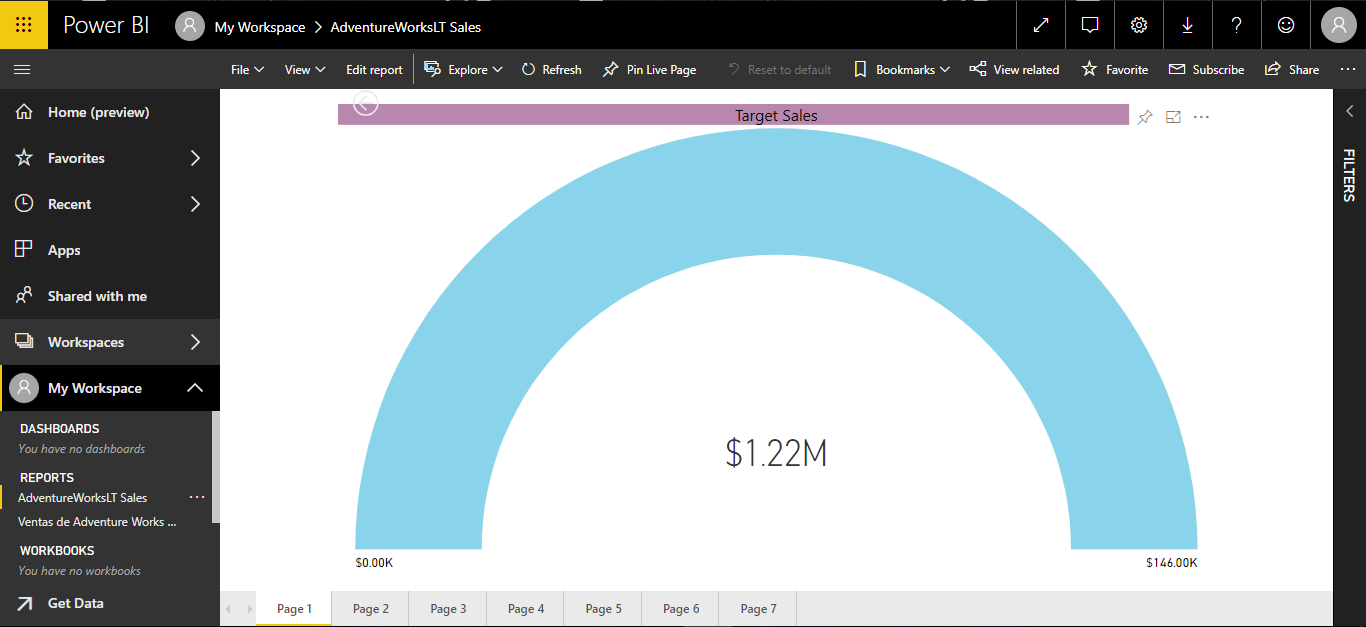
\includegraphics[width=18cm]{./Imagenes/EJER3T2(1)}
	\end{center}	

	\begin{center}
	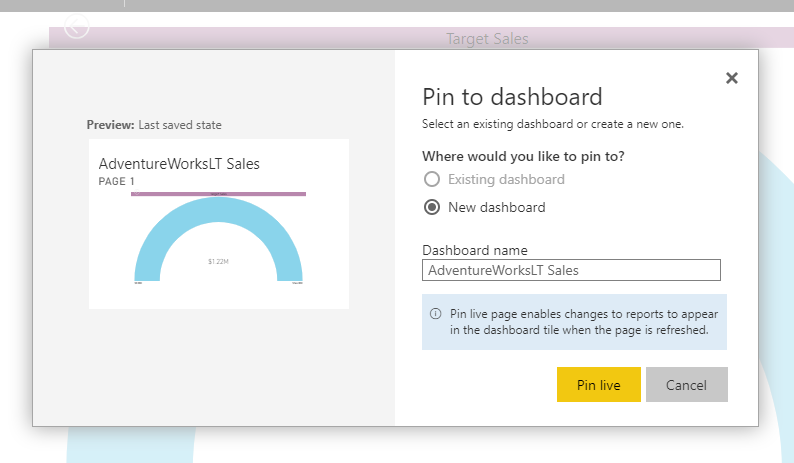
\includegraphics[width=18cm]{./Imagenes/EJER3T2(2)}
	\end{center}	

	\begin{center}
	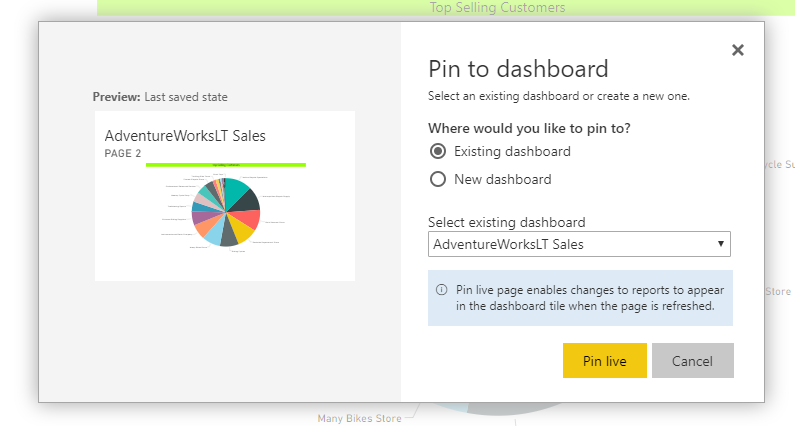
\includegraphics[width=18cm]{./Imagenes/EJER3T2(3)}
	\end{center}	

	\begin{center}
	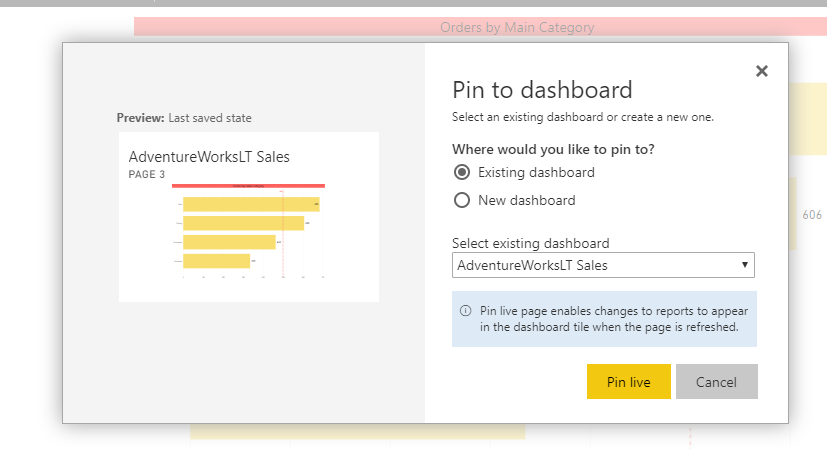
\includegraphics[width=18cm]{./Imagenes/EJER3T2(4)}
	\end{center}	

	\begin{center}
	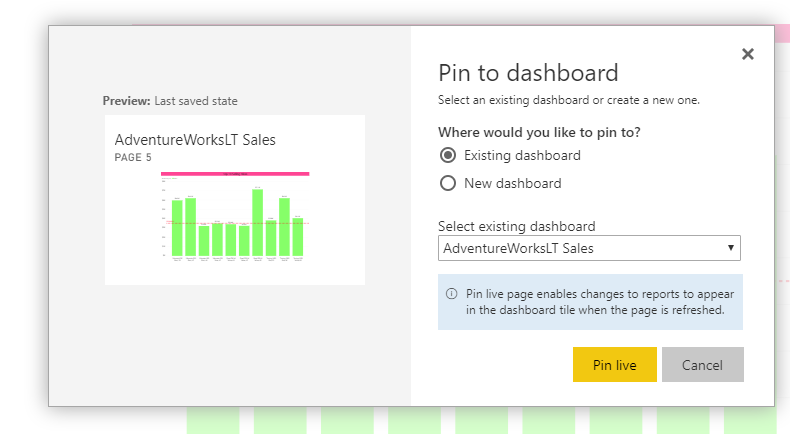
\includegraphics[width=18cm]{./Imagenes/EJER3T2(5)}
	\end{center}	

	\begin{center}
	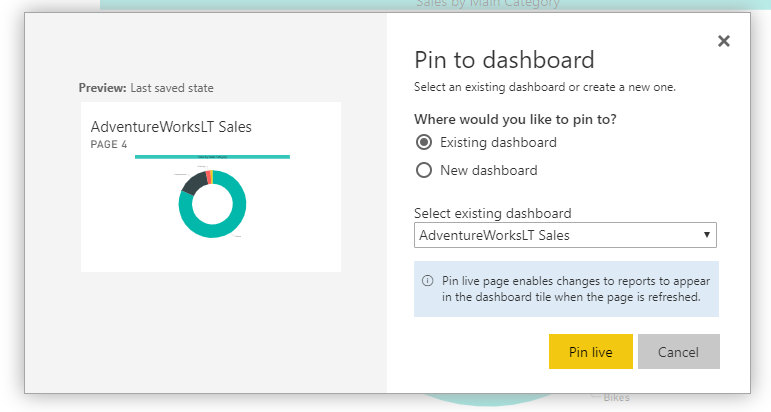
\includegraphics[width=18cm]{./Imagenes/EJER3T2(6)}
	\end{center}	


\end{document}
